\documentclass[]{article}
\usepackage{lmodern}
\usepackage{amssymb,amsmath}
\usepackage{ifxetex,ifluatex}
\usepackage{fixltx2e} % provides \textsubscript
\ifnum 0\ifxetex 1\fi\ifluatex 1\fi=0 % if pdftex
  \usepackage[T1]{fontenc}
  \usepackage[utf8]{inputenc}
\else % if luatex or xelatex
  \ifxetex
    \usepackage{mathspec}
  \else
    \usepackage{fontspec}
  \fi
  \defaultfontfeatures{Ligatures=TeX,Scale=MatchLowercase}
\fi
% use upquote if available, for straight quotes in verbatim environments
\IfFileExists{upquote.sty}{\usepackage{upquote}}{}
% use microtype if available
\IfFileExists{microtype.sty}{%
\usepackage{microtype}
\UseMicrotypeSet[protrusion]{basicmath} % disable protrusion for tt fonts
}{}
\usepackage[margin=1in]{geometry}
\usepackage{hyperref}
\hypersetup{unicode=true,
            pdftitle={MAP 531: Homework},
            pdfauthor={Paul-Antoine GIRARD \& Adrien TOULOUSE},
            pdfborder={0 0 0},
            breaklinks=true}
\urlstyle{same}  % don't use monospace font for urls
\usepackage{color}
\usepackage{fancyvrb}
\newcommand{\VerbBar}{|}
\newcommand{\VERB}{\Verb[commandchars=\\\{\}]}
\DefineVerbatimEnvironment{Highlighting}{Verbatim}{commandchars=\\\{\}}
% Add ',fontsize=\small' for more characters per line
\usepackage{framed}
\definecolor{shadecolor}{RGB}{248,248,248}
\newenvironment{Shaded}{\begin{snugshade}}{\end{snugshade}}
\newcommand{\AlertTok}[1]{\textcolor[rgb]{0.94,0.16,0.16}{#1}}
\newcommand{\AnnotationTok}[1]{\textcolor[rgb]{0.56,0.35,0.01}{\textbf{\textit{#1}}}}
\newcommand{\AttributeTok}[1]{\textcolor[rgb]{0.77,0.63,0.00}{#1}}
\newcommand{\BaseNTok}[1]{\textcolor[rgb]{0.00,0.00,0.81}{#1}}
\newcommand{\BuiltInTok}[1]{#1}
\newcommand{\CharTok}[1]{\textcolor[rgb]{0.31,0.60,0.02}{#1}}
\newcommand{\CommentTok}[1]{\textcolor[rgb]{0.56,0.35,0.01}{\textit{#1}}}
\newcommand{\CommentVarTok}[1]{\textcolor[rgb]{0.56,0.35,0.01}{\textbf{\textit{#1}}}}
\newcommand{\ConstantTok}[1]{\textcolor[rgb]{0.00,0.00,0.00}{#1}}
\newcommand{\ControlFlowTok}[1]{\textcolor[rgb]{0.13,0.29,0.53}{\textbf{#1}}}
\newcommand{\DataTypeTok}[1]{\textcolor[rgb]{0.13,0.29,0.53}{#1}}
\newcommand{\DecValTok}[1]{\textcolor[rgb]{0.00,0.00,0.81}{#1}}
\newcommand{\DocumentationTok}[1]{\textcolor[rgb]{0.56,0.35,0.01}{\textbf{\textit{#1}}}}
\newcommand{\ErrorTok}[1]{\textcolor[rgb]{0.64,0.00,0.00}{\textbf{#1}}}
\newcommand{\ExtensionTok}[1]{#1}
\newcommand{\FloatTok}[1]{\textcolor[rgb]{0.00,0.00,0.81}{#1}}
\newcommand{\FunctionTok}[1]{\textcolor[rgb]{0.00,0.00,0.00}{#1}}
\newcommand{\ImportTok}[1]{#1}
\newcommand{\InformationTok}[1]{\textcolor[rgb]{0.56,0.35,0.01}{\textbf{\textit{#1}}}}
\newcommand{\KeywordTok}[1]{\textcolor[rgb]{0.13,0.29,0.53}{\textbf{#1}}}
\newcommand{\NormalTok}[1]{#1}
\newcommand{\OperatorTok}[1]{\textcolor[rgb]{0.81,0.36,0.00}{\textbf{#1}}}
\newcommand{\OtherTok}[1]{\textcolor[rgb]{0.56,0.35,0.01}{#1}}
\newcommand{\PreprocessorTok}[1]{\textcolor[rgb]{0.56,0.35,0.01}{\textit{#1}}}
\newcommand{\RegionMarkerTok}[1]{#1}
\newcommand{\SpecialCharTok}[1]{\textcolor[rgb]{0.00,0.00,0.00}{#1}}
\newcommand{\SpecialStringTok}[1]{\textcolor[rgb]{0.31,0.60,0.02}{#1}}
\newcommand{\StringTok}[1]{\textcolor[rgb]{0.31,0.60,0.02}{#1}}
\newcommand{\VariableTok}[1]{\textcolor[rgb]{0.00,0.00,0.00}{#1}}
\newcommand{\VerbatimStringTok}[1]{\textcolor[rgb]{0.31,0.60,0.02}{#1}}
\newcommand{\WarningTok}[1]{\textcolor[rgb]{0.56,0.35,0.01}{\textbf{\textit{#1}}}}
\usepackage{graphicx,grffile}
\makeatletter
\def\maxwidth{\ifdim\Gin@nat@width>\linewidth\linewidth\else\Gin@nat@width\fi}
\def\maxheight{\ifdim\Gin@nat@height>\textheight\textheight\else\Gin@nat@height\fi}
\makeatother
% Scale images if necessary, so that they will not overflow the page
% margins by default, and it is still possible to overwrite the defaults
% using explicit options in \includegraphics[width, height, ...]{}
\setkeys{Gin}{width=\maxwidth,height=\maxheight,keepaspectratio}
\IfFileExists{parskip.sty}{%
\usepackage{parskip}
}{% else
\setlength{\parindent}{0pt}
\setlength{\parskip}{6pt plus 2pt minus 1pt}
}
\setlength{\emergencystretch}{3em}  % prevent overfull lines
\providecommand{\tightlist}{%
  \setlength{\itemsep}{0pt}\setlength{\parskip}{0pt}}
\setcounter{secnumdepth}{0}
% Redefines (sub)paragraphs to behave more like sections
\ifx\paragraph\undefined\else
\let\oldparagraph\paragraph
\renewcommand{\paragraph}[1]{\oldparagraph{#1}\mbox{}}
\fi
\ifx\subparagraph\undefined\else
\let\oldsubparagraph\subparagraph
\renewcommand{\subparagraph}[1]{\oldsubparagraph{#1}\mbox{}}
\fi

%%% Use protect on footnotes to avoid problems with footnotes in titles
\let\rmarkdownfootnote\footnote%
\def\footnote{\protect\rmarkdownfootnote}

%%% Change title format to be more compact
\usepackage{titling}

% Create subtitle command for use in maketitle
\providecommand{\subtitle}[1]{
  \posttitle{
    \begin{center}\large#1\end{center}
    }
}

\setlength{\droptitle}{-2em}

  \title{MAP 531: Homework}
    \pretitle{\vspace{\droptitle}\centering\huge}
  \posttitle{\par}
    \author{Paul-Antoine GIRARD \& Adrien TOULOUSE}
    \preauthor{\centering\large\emph}
  \postauthor{\par}
    \date{}
    \predate{}\postdate{}
  
\usepackage{booktabs}
\usepackage{longtable}
\usepackage{array}
\usepackage{multirow}
\usepackage{wrapfig}
\usepackage{float}
\usepackage{colortbl}
\usepackage{pdflscape}
\usepackage{tabu}
\usepackage{threeparttable}
\usepackage{threeparttablex}
\usepackage[normalem]{ulem}
\usepackage{makecell}
\usepackage{xcolor}

\usepackage{dsfont}

\begin{document}
\maketitle

\hypertarget{problem-1-estimating-parameters-of-a-poisson-distribution}{%
\section{Problem 1: Estimating parameters of a Poisson
distribution}\label{problem-1-estimating-parameters-of-a-poisson-distribution}}

We recall that the Poisson distribution with parameter \(\theta > 0\)
has a pdf given by (\(p(\theta, k), k \in \mathbb{N})\) w.r.t the
counting measure on \(\mathbb{N}\):\\
\[p(\theta, k) = e^{-\theta} \frac{\theta^k}{k!}\]

\hypertarget{question-1}{%
\subsubsection{Question 1}\label{question-1}}

The poisson distribution is a discrete distribution since it has a
countable number of possible values (\(\mathbb{N}\)).

In statistics, we use this distribution to compute the probability of a
given number of (rare) events in a time period.

For example a poisson distribution can model:

\begin{itemize}
\item
  The number of patients arriving in an emergency room between 9 and
  10am.
\item
  The number of network failures per day.
\item
  In quality control, the number of manufacturing defect.
\end{itemize}

\hypertarget{question-2}{%
\subsubsection{Question 2}\label{question-2}}

We assume that \(\mathbb{X}\) follows a Poisson distribution with
parameter \(\theta > 0\).

We will use the fact that
\(e^{\theta} = \sum_{i=0}^{\infty} (\frac{\theta^{i}}{i!}), \forall \theta \in \mathbb{R}\)
\[
\mathbb{E}[\mathbb{X}] = \sum_{i=0}^{\infty} (i * p(\theta, i)) = \sum_{i=0}^{\infty} (i*e^{-\theta} \frac{\theta^{i}}{i!}) = \theta * e^{-\theta}\sum_{i=1}^{\infty} (\frac{\theta^{i-1}}{(i-1)!}) = \theta * e^{-\theta} \sum_{i=0}^{\infty} (\frac{\theta^{i}}{i!}) = \theta * e^{-\theta} * e^{\theta} = \theta  
\]

\[
\mathbb{E}[\mathbb{X}^2] = \sum_{i=0}^{\infty} (i^2 * p(\theta, i)) = \sum_{i=0}^{\infty} (i^2*e^{-\theta} \frac{\theta^{i}}{i!}) = \theta * e^{-\theta}\sum_{i=1}^{\infty} (i\frac{\theta^{i-1}}{(i-1)!}) = \theta * e^{-\theta}\sum_{i=0}^{\infty} ((i+1)\frac{\theta^{i}}{i!})
\] \[
= \theta * e^{-\theta}[\sum_{i=0}^{\infty} (i\frac{\theta^{i}}{i!}) + \sum_{i=0}^{\infty} (\frac{\theta^{i}}{i!})] = \theta * e^{-\theta}[\theta \sum_{i=0}^{\infty} (\frac{\theta^{i}}{i!}) + e^{\theta}] = \theta * e^{-\theta}[\theta * e^{\theta} + e^{\theta}] = \theta (\theta + 1)
\]

\[
\mathbb{V} (\mathbb{X}) = \mathbb{E}[\mathbb{X}^2] - \mathbb{E}[\mathbb{X}]^2 = \theta (\theta + 1) - \theta^2 = \theta
\]

\hypertarget{question-3}{%
\subsubsection{Question 3}\label{question-3}}

We are provided with n independent observations of a Poisson random
variable of parameter \(\theta \in \Theta = \mathbb{R_+^*}\). Our
observations are
\(X_k \sim Pois (\theta), \forall k \in {1, ..., n}\).\\
The corresponding statistical model is:
\[\mathcal{M}^n = (\mathbb{N}^n, \mathcal{P}(\mathbb{N}^n),\ \{\mathbb{P}^n _{\theta},\ \theta \in\Theta \})\]
with
\(\mathbb{P}^n _{\theta} = \mathbb{P} _{\theta} \otimes ... \otimes \mathbb{P} _{\theta}\)
(n times)\\
We are trying to estimate the parameter \(\theta\).

\hypertarget{question-4}{%
\subsubsection{Question 4}\label{question-4}}

The likelihood function is the function on \(\theta\) that makes our n
observations most likely.

Using the independance of the \(X_k\): \[
l(\theta) = \prod_{k=1}^{n} e^{-\theta} \frac{\theta^{X_{k}}}{X_{k}!}
\]

\[
L(\theta) = log(l(\theta)) = \sum_{k=1} ^{n}(- \theta + X_k log(\theta) - log(X_k!)) = - n \theta + log(\theta) \sum_{k=1}^{n}X_{k} - \sum_{k=1}^{n}log(X_{k}!)
\]

By derivating with respect to \(\theta\), we have:

\[
L'(\theta) = -n +\frac{\sum_{k=1}^{n}X_{k}}{\theta}
\] \[
L''(\theta) = - \frac{\sum_{k=1}^{n}X_{k}}{\theta^2} < 0
\] Since, the second derivative of the log-likelihood function is
negative, the function is concave and admits a global maximum given by:
\[
L'(\theta) = 0 \Leftrightarrow -n +\frac{\sum_{k=1}^{n}X_{k}}{\theta} = 0 \Leftrightarrow \hat\theta_{MLE} = \overline{X}
\]

So, the maximum likelihood estimator is: \[
\hat\theta_{MLE} = \overline{X}
\]

\hypertarget{question-5}{%
\subsubsection{Question 5}\label{question-5}}

Since the \(X_k\) are iid, we have that: \[
\mathbb{E}[\overline{X}] = \frac{1}{n} \sum _{k = 1} ^{n} \mathbb{E} [X_k] = \mathbb{E} [X_1] = \theta
\]

\[
\mathbb{V}(\overline{X}) = \frac{1}{n^2} \sum _{k = 1} ^{n} \mathbb{V} (X_k) = \frac{1}{n} \mathbb{V} [X_1] = \frac {\theta} {n}
\] Applying the central limit theorem, we have that
\(\sqrt{n}(\hat\theta_{MLE}-\theta)\) converges towards a Gaussian
\(\mathcal{N}(0,\theta)\).

\hypertarget{question-6}{%
\subsubsection{Question 6}\label{question-6}}

The weak law of large numbers gives us that \(\hat\theta_{MLE}\)
converges in probability towards \(\theta\).\\
By continuous mapping, \(\sqrt{\hat\theta_{MLE}}\) converges in
probability towards \(\sqrt{\theta}\). Then, by Slutsky's theorem, we
have that
\(\sqrt{n}\frac{(\hat\theta_{MLE}-\theta)}{\sqrt{\hat\theta_{MLE}}}\)
converges in law towards a gaussian \(\mathcal{N}(0,1)\).

Let's check this result in R by simulating 1000 times our random
variable
\(\sqrt{n}\frac{(\hat\theta_{MLE}-\theta)}{\sqrt{\hat\theta_{MLE}}}\)
with a sample size of 100:

\begin{Shaded}
\begin{Highlighting}[]
\NormalTok{estim <-}\StringTok{ }\ControlFlowTok{function}\NormalTok{(x, theta)\{}
\NormalTok{  n <-}\StringTok{ }\KeywordTok{length}\NormalTok{(x)}
\NormalTok{  est <-}\StringTok{ }\KeywordTok{sqrt}\NormalTok{(n) }\OperatorTok{*}\StringTok{ }\NormalTok{(}\KeywordTok{mean}\NormalTok{(x) }\OperatorTok{-}\StringTok{ }\NormalTok{theta) }\OperatorTok{/}\StringTok{ }\KeywordTok{sqrt}\NormalTok{(}\KeywordTok{mean}\NormalTok{(x))}
  \KeywordTok{return}\NormalTok{(est)\}}
\end{Highlighting}
\end{Shaded}

\begin{Shaded}
\begin{Highlighting}[]
\KeywordTok{set.seed}\NormalTok{(}\DecValTok{42}\NormalTok{)}
\NormalTok{Nattempts =}\StringTok{ }\FloatTok{1e3}
\NormalTok{nsample =}\StringTok{ }\DecValTok{100}
\NormalTok{theta =}\StringTok{ }\DecValTok{3}

\NormalTok{samples <-}\StringTok{ }\KeywordTok{lapply}\NormalTok{(}\DecValTok{1}\OperatorTok{:}\NormalTok{Nattempts, }\ControlFlowTok{function}\NormalTok{(i) }\KeywordTok{rpois}\NormalTok{(nsample, theta))}
\NormalTok{realisations <-}\StringTok{ }\KeywordTok{sapply}\NormalTok{(samples, }\ControlFlowTok{function}\NormalTok{(x) }\KeywordTok{estim}\NormalTok{(x, theta))}

\KeywordTok{hist}\NormalTok{(realisations, }\DataTypeTok{probability =} \OtherTok{TRUE}\NormalTok{)}
\NormalTok{d =}\StringTok{ }\KeywordTok{density}\NormalTok{(realisations, }\DataTypeTok{kernel=}\StringTok{'gaussian'}\NormalTok{)}
\KeywordTok{lines}\NormalTok{(d, }\DataTypeTok{col =} \StringTok{'red'}\NormalTok{)}
\end{Highlighting}
\end{Shaded}

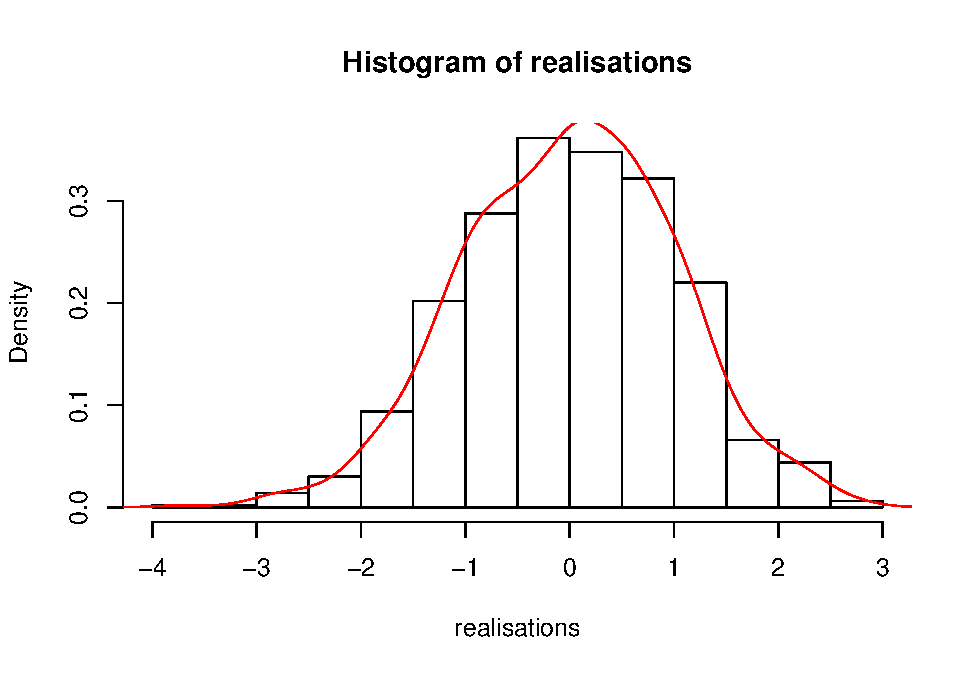
\includegraphics{Homework_Adrien_Toulouse_Paul-Antoine_Girard_files/figure-latex/unnamed-chunk-2-1.pdf}

\begin{Shaded}
\begin{Highlighting}[]
\KeywordTok{qqnorm}\NormalTok{(realisations)}
\KeywordTok{qqline}\NormalTok{(realisations)}
\end{Highlighting}
\end{Shaded}

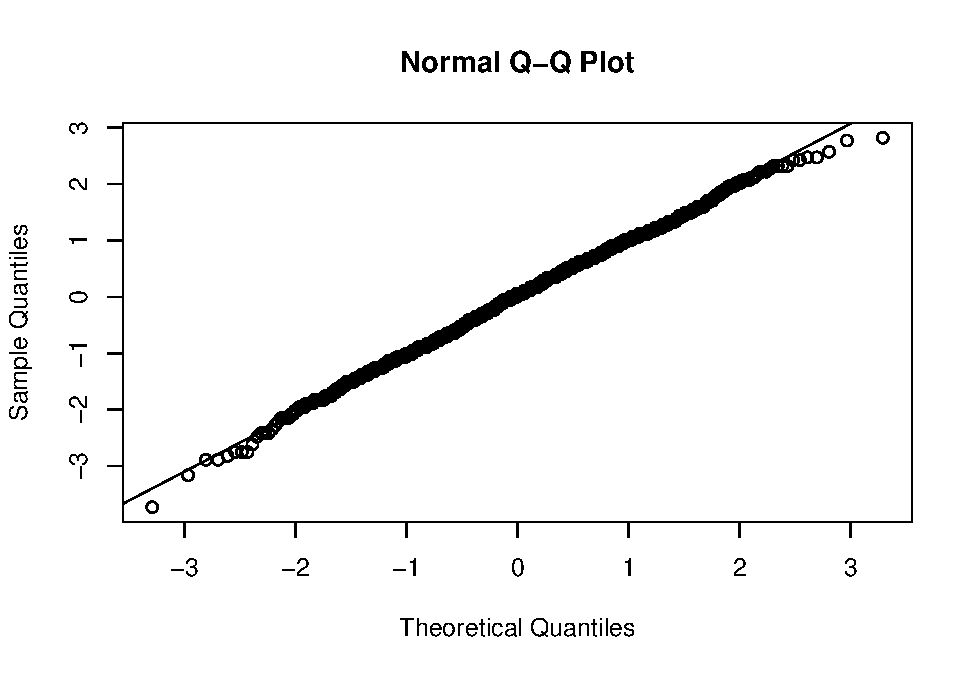
\includegraphics{Homework_Adrien_Toulouse_Paul-Antoine_Girard_files/figure-latex/unnamed-chunk-3-1.pdf}

This confirms what we found theoretically: the random variable
\(\sqrt{n}\frac{(\hat\theta_{MLE}-\theta)}{\sqrt{\hat\theta_{MLE}}}\)
follows a standard gaussian distribution.

\hypertarget{question-7}{%
\subsubsection{Question 7}\label{question-7}}

Let
\(Z_n = \sqrt{n} \frac{(\hat\theta_{MLE}-\theta)}{\sqrt{\hat\theta_{MLE}}}\)
be our random variable.

Denote \(z_{alpha}\) the \(\alpha\)-quantile for the standard Normal
distribution for \(\alpha \in (0,\ 1)\).

\[
\lim \limits_{n \rightarrow + \infty} \mathbb{P} (-z_{1-\alpha/2} \leq Z_n \leq z_{1-\alpha/2}) \ge 1- \alpha \Leftrightarrow \lim \limits_{n \rightarrow + \infty} \mathbb{P}(-z_{1-\alpha/2} \sqrt{\frac{\hat\theta_{MLE}}{n}} \leq \hat\theta_{MLE} - \theta \leq z_{1-\alpha/2}\sqrt{\frac{\hat\theta_{MLE}}{n}}) \ge 1- \alpha
\]

For \(\alpha \in (0, 1)\), an asymptotic confidence interval for
\(\theta\) of level \(\alpha\) is therefore :

\[
[\hat \theta_{MLE} - z_{1-\alpha/2} \frac{\sqrt{\hat\theta_{MLE}}}{\sqrt{n}} ;\ \hat \theta_{MLE} + z_{1-\alpha/2} \frac{\sqrt{\hat\theta_{MLE}}} {\sqrt{n}}]
\]

\hypertarget{question-8}{%
\subsubsection{Question 8}\label{question-8}}

We apply the \(\delta\)-method with \(g(x) = 2 \sqrt{x}\)\\
We have: \(g'(x) = \frac {1} {\sqrt{x}}\)\\
So, \[
\sqrt{n} (g(\hat \theta_{MLE}) - g(\theta)) \overset{d} {\to} \mathcal{N}(0,\ g'(\theta)^2 \times \theta) \Leftrightarrow \sqrt{n} (g(\hat \theta_{MLE}) - g(\theta)) \overset{d} {\to} \mathcal{N}(0,1)
\]

\hypertarget{question-9}{%
\subsubsection{Question 9}\label{question-9}}

Let \(W_n = \sqrt{n} (2 \sqrt{\hat\theta_{MLE}} - 2 \sqrt{\theta})\) be
our random variable.

We know by the last question that
\(W_n \overset{d} {\to} \mathcal{N}(0,1)\). \[
\lim \limits_{n \rightarrow + \infty} \mathbb{P} (-z_{1-\alpha/2} \leq W_n \leq z_{1-\alpha/2}) \geq 1- \alpha \Leftrightarrow \lim \limits_{n \rightarrow + \infty} \mathbb{P}(- \frac {z_{1-\alpha/2}} {2 \sqrt{n}} \leq \sqrt{\hat\theta_{MLE}} - \sqrt{\theta} \leq \frac {z_{1-\alpha/2}} {2 \sqrt{n}}) \geq 1- \alpha
\]

\[
 \Leftrightarrow \lim \limits_{n \rightarrow + \infty} \mathbb{P} (\sqrt{\hat\theta_{MLE}} - \frac {z_{1-\alpha/2}} {2 \sqrt{n}} \leq \sqrt{\theta} \leq \sqrt{\hat\theta_{MLE}} + \frac {z_{1-\alpha/2}} {2 \sqrt{n}}) \geq 1- \alpha
\] When n goes towards infinity, \(\frac {z_{1-\alpha/2}} {2 \sqrt{n}}\)
goes to 0. Since \(\sqrt{\hat\theta_{MLE}}\) is positive, there exists a
\(n_0\) such that
\(\sqrt{\hat\theta_{MLE}} - \frac {z_{1-\alpha/2}} {2 \sqrt{n}}\) is
positive and we can take the squares in the inequality without changing
the order of the inequalities:

\[
\Leftrightarrow \lim \limits_{n \rightarrow + \infty} \mathbb{P} ((\sqrt{\hat\theta_{MLE}} - \frac {z_{1-\alpha/2}} {2 \sqrt{n}})^2 \leq \theta \leq (\sqrt{\hat\theta_{MLE}} + \frac {z_{1-\alpha/2}} {2 \sqrt{n}})^2) \geq 1- \alpha
\]

For \(\alpha \in (0, 1)\), an asymptotic confidence interval for
\(\theta\) of level \(\alpha\) is therefore: \[
[(\sqrt{\hat\theta_{MLE}} - \frac {z_{1-\alpha/2}} {2 \sqrt{n}})^2 ;\ (\sqrt{\hat\theta_{MLE}} + \frac {z_{1-\alpha/2}} {2 \sqrt{n}})^2]
\]

\hypertarget{question-10}{%
\subsubsection{Question 10}\label{question-10}}

Based on the first moment of a poisson distribution, we easily have
that:

\[\hat \theta_{MME} = \overline{X}\]

We can remark that \(\hat \theta_{MME} = \hat \theta_{MLE}\)

Based on the second moment of a poisson distribution, we have:
\[n^{-1} \sum _{k=1} ^{n} X_k^2 = \hat \theta_{2} (\hat \theta_{2} + 1)\]

Let's define the function \(h(x) = x(x + 1)\)\\
Its inverse on \(\mathbb{R}_+^*\) is
\(h^{-1} (x) = \frac {1}{2} [- 1 + \sqrt{4 x + 1}]\) and this gives us:
\[\hat \theta_{2} = \frac {1}{2} [- 1 + \sqrt{(4 n^{-1} \sum _{k=1} ^{n} X_k^2) + 1}]\]

\hypertarget{question-11}{%
\subsubsection{Question 11}\label{question-11}}

\(\mathbb{E} [\hat\theta_{MLE}] = \frac{1}{n} \sum_{k=1}^{n} \mathbb{E}[X_k]\)
by linearity of the expectation. So,
\[\mathbb{E} [\hat\theta_{MLE}] = \frac{1}{n} * n * \theta = \theta\]

Therefore, \(\hat\theta_{MLE}\) is an unbiased estimator of \(\theta\),
ie. \(b_\theta{^*}(\hat\theta_{MLE}) = 0\)

\(\mathbb{V} (\hat\theta_{MLE}) = \frac{1}{n^2} \sum_{i=1}^{n} \mathbb{V}(X_i)\)
by independance of the \(X_k\).
\[\mathbb{V} (\hat\theta_{MLE}) = \frac{1}{n^2} * n * \theta = \frac{\theta}{n}\]

The quadratic risk Q is:
\[Q = b_\theta{^*}(\hat\theta_{MLE})^2 + \mathbb{V^*} (\hat\theta_{MLE}) = 0 + \frac{\theta}{n} = \frac{\theta}{n}\]

\hypertarget{question-12}{%
\subsubsection{Question 12}\label{question-12}}

\(\hat\theta_{MLE}\) is an unbiased estimator. So the Cramer-Rao bound
is given by:\\
\[\frac{1}{I_n(\theta^*)} = \frac{1}{\mathbb{E} [-L''(\theta^*)]}\]

By derivating the log-likelihood function with respect to \(\theta\), we
have: \[L'(\theta^*) = -n + \frac{\sum_{i=1}^{n} X_k}{\theta}\]
\[-L''(\theta^*) = \frac{\sum_{i=1}^{n} X_k}{\theta^2}\]

Therefore,
\[\mathbb{E} [-L''(\theta^*)] = \frac{\sum_{i=1}^{n} \mathbb{E}[X_k]}{\theta^2} = \frac{n}{\theta}\]

Finally,
\[\frac{1}{I_n(\theta^*)} = \frac{\theta}{n} = \mathbb{V} (\hat\theta_{MLE})\]

We can conclude that our estimator \(\hat\theta_{MLE}\) is efficient.

\hypertarget{question-13}{%
\subsubsection{Question 13}\label{question-13}}

\[
\hat\theta_{2} = \frac{1}{n} \sum_{i=1}^{n} (X_i - \overline{X_n})^2 = \frac{1}{n} \sum_{i=1}^{n} (X_i - \theta + \theta - \overline{X_n})^2 = \frac{1}{n} \sum_{i=1}^{n} [(X_i - \theta)^2 + (\theta - \overline{X_n} )^2 +2(X_i - \theta)(\theta - \overline{X_n})]
\] \[
= \frac{1}{n} \sum_{i=1}^{n} (X_i - \theta)^2 + (\theta - \overline{X_n} )^2  + \frac{2}{n}(\theta - \overline{X_n}) \sum_{i=1}^{n}(X_i - \theta) \\
= \frac{1}{n} \sum_{i=1}^{n} (X_i - \theta)^2 + (\theta - \overline{X_n} )^2 + 2(\theta - \overline{X_n}) (\overline{X_n} - \theta )
\] \[
= \frac{1}{n} \sum_{i=1}^{n} (X_i - \theta)^2 - (\theta - \overline{X_n})^2
\]

\hypertarget{question-14}{%
\subsubsection{Question 14}\label{question-14}}

\[
\mathbb{E}[(\theta - \overline{X_n})^2] = \mathbb{E}[\theta^2 - 2\theta\overline{X_n} + \overline{X_n}^2] = \theta^2 - 2\theta\mathbb{E}[\overline{X_n}] + \mathbb{E}[\overline{X_n^2}]
\] \[
=- \theta^2 + \mathbb{V}(\overline{X_n}) + \mathbb{E}[\overline{X_n}^2] = - \theta^2 + \frac{\theta}{n} + \theta^2 = \frac{\theta}{n}
\]

\[
\mathbb{E}[\hat\theta_2] = \mathbb{E} [\frac{1}{n} \sum_{i=1}^{n} (X_i - \theta)^2 - (\theta - \overline{X_n})^2] = \frac{1}{n} \sum_{i=1}^{n}\mathbb{E}[(X_i - \theta)^2] - \mathbb{E}[(\theta - \overline{X_n})^2]
\]
\[= \frac{1}{n} \sum_{i=1}^{n}\mathbb{V}(X_i) - \frac{\theta}{n} = \theta(1-\frac{1}{n})\]
Therefore the bias is: \[b_{\hat\theta_2} =  -\frac{\theta}{n}\]

We can get an unbiased estimator \(\hat\theta_3\) by defining
\(\hat\theta_3 = (1-\frac{1}{n}) ^{-1} \hat\theta_2\)

\hypertarget{question-15}{%
\subsubsection{Question 15}\label{question-15}}

Using the previous questions, we know that:
\[\hat\theta_{2} = \frac{1}{n} \sum_{i=1}^{n} (X_i - \theta)^2 - (\theta - \overline{X_n})^2\]
therefore, we have: \[
\sqrt{n} (\hat\theta_{2} - \theta) = \frac{1}{\sqrt{n}} \sum_{i=1}^{n} (X_i - \theta)^2 - \sqrt{n} (\theta - \overline{X_n})^2 - \sqrt{n} \theta = \sqrt{n} (\overline{Y_n} - \theta) -  \sqrt{n} (\theta - \overline{X_n})^2
\] where: \[\forall i \in[\![1,n]\!], Yi = (X_i - \theta)^2 \]
\[\bar{Y_n} = \frac{1}{n} \sum_{i=1}^{n}Y_i \]

Since: \[
\mathbb{E}[Y_i] = \mathbb{V}(X_i) = \theta
\] and \[
\mathbb{V}(Y_i) = 2\theta^2 + \theta
\]

We can apply the central limit theorem, and we have that
\[\sqrt{n} (\overline{Y_n} - \theta) \overset{d} {\to} \mathcal{N}(0,2\theta^2 + \theta)\]

We also have that: \[
\sqrt{n} (\theta - \overline{X_n})^2 = \sqrt{n} (\overline{X_n} - \theta)^2 = \sqrt{n} (\overline{X_n} - \theta)(\overline{X_n} - \theta)
\]

Applying the central limit theorem, we have that:
\(\sqrt{n} (\overline{X_n} - \theta) \overset{d} {\to} \mathcal{N}(0,\theta)\).\\
On the other hand, applying the law of large numbers:
\((\theta - \overline{X_n})\overset{p} {\to} 0\).

Applying Slutsky's theorem, \(\sqrt{n} (\theta - \overline{X_n})^2\)
converges in distribution towards the constant 0. Therefore, it
converges in probability towards 0.

Now, we can apply Slutsky's theorem to
\(\sqrt{n} (\overline{Y_n} - \theta) - \sqrt{n} (\theta - \overline{X_n})^2\)
which gives us finally that:
\[\sqrt{n} (\hat\theta_{2} - \theta) \overset{d} {\to} \mathcal{N}(0,2\theta^2 + \theta)\]

We can now compute an other asymptotic confidence interval centered in
\(\hat \theta_2\).

Let
\(V_n = \sqrt{n}\frac{(\hat\theta_{2}-\theta)}{\sqrt{2\hat\theta_{2}^2 + \hat\theta_{2}}}\)
be our random variable.

We know by the first part of question that
\(\frac{V_n}{\sqrt{2\theta^2 + \theta}} \overset{d} {\to} \mathcal{N}(0,1)\).

Let's use \(\hat\theta_{2}\) as an estimator of \(\theta\) for the
denominator. In order to apply slutsky's theorem, we will prove that
\(\hat\theta_{2} \overset{p} {\to} \theta\).

Let \(\epsilon > 0\). By Chebyshev's inequality, \[
P(\mid \hat\theta_{2} - \theta \mid > \epsilon) < \frac{Var(\hat\theta_{2} - \theta)} {\epsilon^2} = \frac{\theta^2 + \theta} {n\epsilon^2} \underset{n \to + \infty} {\to} 0
\]

So, we have that \(\hat\theta_{2} \overset{p} {\to} \theta\) and by
continuous mapping,
\[\sqrt{2\hat\theta_{2}^2 + \hat\theta_{2}} \overset{p} {\to} \sqrt{2\theta^2 + \theta}\]
Then, by Slutsky's theorem, we have that
\(V_n =\sqrt{n}\frac{(\hat\theta_{2}-\theta)}{\sqrt{2\hat\theta_{2}^2 + \hat\theta_{2}}}\)
converges in law towards a gaussian \(\mathcal{N}(0,1)\).

\[
\lim \limits_{n \rightarrow + \infty} \mathbb{P} (-z_{1-\alpha/2} \leq V_n \leq z_{1-\alpha/2}) \geq 1- \alpha \Leftrightarrow \lim \limits_{n \rightarrow + \infty} \mathbb{P}(-z_{1-\alpha/2} \frac{\sqrt{2\hat\theta_{2}^2 + \hat\theta_{2}}} {\sqrt{n}} \leq \hat\theta_{2} - \theta \leq z_{1-\alpha/2} \frac{\sqrt{2\hat\theta_{2}^2 + \hat\theta_{2}}} {\sqrt{n}}) \geq 1- \alpha
\]

\[
 \Leftrightarrow \lim \limits_{n \rightarrow + \infty} \mathbb{P} (\hat\theta_{2} - z_{1-\alpha/2} \frac{\sqrt{2\hat\theta_{2}^2 + \hat\theta_{2}}} {\sqrt{n}} \leq \theta \leq \hat\theta_{2} + z_{1-\alpha/2} \frac{\sqrt{2\hat\theta_{2}^2 + \hat\theta_{2}}} {\sqrt{n}}) \geq 1- \alpha
\]

For \(\alpha \in (0, 1)\), an asymptotic confidence interval for
\(\theta\) of level \(\alpha\) is therefore: \[
[\hat\theta_{2} - z_{1-\alpha/2} \frac{\sqrt{2\hat\theta_{2}^2 + \hat\theta_{2}}} {\sqrt{n}};\ \hat\theta_{2} + z_{1-\alpha/2} \frac{\sqrt{2\hat\theta_{2}^2 + \hat\theta_{2}}} {\sqrt{n}}]
\]

\hypertarget{question-16}{%
\subsubsection{Question 16}\label{question-16}}

Let \(s \in \mathbb{R}\). The probability generating function of the
Poisson distribution is given by: \[
G_\mathbb{X} (s) = \mathbb{E}[exp(s\mathbb{X})] = \sum _{k=0} ^{\infty} e^{ks} e^{-\theta} \frac{\theta^k}{k!} = e^{-\theta} \sum _{k=0} ^{\infty} \frac{(\theta e^s)^k}{k!} = e^{-\theta} e^{\theta e^{s}} = e^{\theta(e^{s}-1)}
\]

In order to compute the first and second moment of the Poisson
distribution, we can now use the moment generating function. Let's
compute its first and second order derivatives.

\[G_\mathbb{X}' (s) = \theta e^{s} e^{\theta (e^{s}-1)}\]
\[G_\mathbb{X}'' (s) = \theta [e^{s} e^{\theta (e^{s}-1)} + \theta e^{2s} e^{\theta (e^{s}-1)}] = \theta e^{s} [e^{\theta (e^{s}-1)} + \theta e^{s} e^{\theta (e^{s}-1)}]\]

Then, we have: \[\mathbb{E} [\mathbb{X}] = G_\mathbb{X}' (0) = \theta\]
\[\mathbb{E} [\mathbb{X}^2] = G_\mathbb{X}'' (0) = \theta(1 + \theta)\]
\[\mathbb{V}(\mathbb{X}) = \mathbb{E} [\mathbb{X}^2] - \mathbb{E} [\mathbb{X}]^2 = \theta(1 + \theta) - \theta^2 = \theta\]

We will now show that:
\(\mathbb{V}[(\mathbb{X}_i - \theta)^2] = 2 \theta^2 + \theta\)

\[G_\mathbb{X}^{(3)} (s) = (1 + 3 \theta e^{s} + \theta^2 e^{2s}) \theta e^{s + \theta (e^{s}-1)}\]
\[G_\mathbb{X}^{(4)} (s) = (1 + \theta^3 e^{3s} + 6 \theta^2 e^{2s} + 7\theta e^{s}) \theta e^{s + \theta (e^{s}-1)}\]
\[\mathbb{E} [\mathbb{X}^3] = G_\mathbb{X}^{(3)} (0) = \theta + 3\theta^2 + \theta^3\]
\[\mathbb{E} [\mathbb{X}^4] = G_\mathbb{X}^{(4)} (0) = \theta^4 + 6\theta^3 + 7\theta^2 + \theta\]
\[
\mathbb{V}[(\mathbb{X}_i - \theta)^2] = \mathbb{E} [(\mathbb{X} - \theta)^4] - \mathbb{E} [(\mathbb{X} - \theta)^2]^2 = \mathbb{E} [\mathbb{X}^4] - 4 \theta \mathbb{E} [\mathbb{X}^3] + 6 \theta^2 \mathbb{E} [\mathbb{X}^2]  - 4 \theta^3 \mathbb{E} [\mathbb{X}] + \theta^4 - Var (\mathbb{X})^2
\] \[
= \theta^4 + 6\theta^3 + 7\theta^2 + \theta - 4\theta (\theta + 3\theta^2 + \theta^3) + 6 \theta^2 (\theta +\theta^2) - 4\theta^4  + \theta^4 - \theta^2 = 2 \theta^2 + \theta
\]

\hypertarget{problem-2-analysis-of-the-usjudgeratings-dataset}{%
\section{Problem 2: Analysis of the USJudgeRatings
dataset}\label{problem-2-analysis-of-the-usjudgeratings-dataset}}

This exercise is open. You are asked to use the tools we have seen
together to analyze the USJudgeRatings data set. This data set is
provided in the package datasets. Your analysis should be reported here
and include:

\begin{itemize}
\tightlist
\item
  an introduction
\item
  a general description of the data
\item
  the use of descriptive statistics
\item
  the use of all techniques we have seen together that might be relevant
\item
  a conclusion
\end{itemize}

Overall, your analysis, including the graphs and the codes should not
exceed 15 pages in pdf.

\hypertarget{introduction}{%
\subsection{Introduction}\label{introduction}}

We are given to analyse a dataset, named USJudgeratings, containing
various ratings of state judges in the US Superior Court made by
lawyers. The different variables given help us to determine if a judge
is worthy staying in the US Superior Court or not. We will start by
doing a general description of the data and applying descriptive
statistics to better apprehend the data.

\hypertarget{general-description}{%
\subsection{General description}\label{general-description}}

We start by uploading our data.

\begin{Shaded}
\begin{Highlighting}[]
\KeywordTok{data}\NormalTok{(USJudgeRatings)}
\end{Highlighting}
\end{Shaded}

First, let's see how the dataset is organized.

\begin{Shaded}
\begin{Highlighting}[]
\KeywordTok{str}\NormalTok{(USJudgeRatings)}
\end{Highlighting}
\end{Shaded}

\begin{verbatim}
## 'data.frame':    43 obs. of  12 variables:
##  $ CONT: num  5.7 6.8 7.2 6.8 7.3 6.2 10.6 7 7.3 8.2 ...
##  $ INTG: num  7.9 8.9 8.1 8.8 6.4 8.8 9 5.9 8.9 7.9 ...
##  $ DMNR: num  7.7 8.8 7.8 8.5 4.3 8.7 8.9 4.9 8.9 6.7 ...
##  $ DILG: num  7.3 8.5 7.8 8.8 6.5 8.5 8.7 5.1 8.7 8.1 ...
##  $ CFMG: num  7.1 7.8 7.5 8.3 6 7.9 8.5 5.4 8.6 7.9 ...
##  $ DECI: num  7.4 8.1 7.6 8.5 6.2 8 8.5 5.9 8.5 8 ...
##  $ PREP: num  7.1 8 7.5 8.7 5.7 8.1 8.5 4.8 8.4 7.9 ...
##  $ FAMI: num  7.1 8 7.5 8.7 5.7 8 8.5 5.1 8.4 8.1 ...
##  $ ORAL: num  7.1 7.8 7.3 8.4 5.1 8 8.6 4.7 8.4 7.7 ...
##  $ WRIT: num  7 7.9 7.4 8.5 5.3 8 8.4 4.9 8.5 7.8 ...
##  $ PHYS: num  8.3 8.5 7.9 8.8 5.5 8.6 9.1 6.8 8.8 8.5 ...
##  $ RTEN: num  7.8 8.7 7.8 8.7 4.8 8.6 9 5 8.8 7.9 ...
\end{verbatim}

The data is stored in a dataframe.

\begin{Shaded}
\begin{Highlighting}[]
\KeywordTok{dim}\NormalTok{(USJudgeRatings)}
\end{Highlighting}
\end{Shaded}

\begin{verbatim}
## [1] 43 12
\end{verbatim}

We are provided with n = 43 observations and p = 12 quantitative
variables.

We can have a full view of the dataset by using the kable function:

\begin{Shaded}
\begin{Highlighting}[]
\KeywordTok{library}\NormalTok{(knitr)}
\KeywordTok{library}\NormalTok{(kableExtra)}
\KeywordTok{kable}\NormalTok{(USJudgeRatings, }\StringTok{'latex'}\NormalTok{, }\DataTypeTok{caption =} \StringTok{"Ratings of US judges"}\NormalTok{, }\DataTypeTok{booktabs =}\NormalTok{ T) }\OperatorTok
\StringTok{  }\KeywordTok{kable_styling}\NormalTok{(}\DataTypeTok{latex_options =} \StringTok{"striped"}\NormalTok{, }\DataTypeTok{font_size =} \DecValTok{6}\NormalTok{)}
\end{Highlighting}
\end{Shaded}

\begin{table}

\caption{\label{tab:view}Ratings of US judges}
\centering
\fontsize{6}{8}\selectfont
\begin{tabular}[t]{lrrrrrrrrrrrr}
\toprule
  & CONT & INTG & DMNR & DILG & CFMG & DECI & PREP & FAMI & ORAL & WRIT & PHYS & RTEN\\
\midrule
\rowcolor{gray!6}  AARONSON,L.H. & 5.7 & 7.9 & 7.7 & 7.3 & 7.1 & 7.4 & 7.1 & 7.1 & 7.1 & 7.0 & 8.3 & 7.8\\
ALEXANDER,J.M. & 6.8 & 8.9 & 8.8 & 8.5 & 7.8 & 8.1 & 8.0 & 8.0 & 7.8 & 7.9 & 8.5 & 8.7\\
\rowcolor{gray!6}  ARMENTANO,A.J. & 7.2 & 8.1 & 7.8 & 7.8 & 7.5 & 7.6 & 7.5 & 7.5 & 7.3 & 7.4 & 7.9 & 7.8\\
BERDON,R.I. & 6.8 & 8.8 & 8.5 & 8.8 & 8.3 & 8.5 & 8.7 & 8.7 & 8.4 & 8.5 & 8.8 & 8.7\\
\rowcolor{gray!6}  BRACKEN,J.J. & 7.3 & 6.4 & 4.3 & 6.5 & 6.0 & 6.2 & 5.7 & 5.7 & 5.1 & 5.3 & 5.5 & 4.8\\
\addlinespace
BURNS,E.B. & 6.2 & 8.8 & 8.7 & 8.5 & 7.9 & 8.0 & 8.1 & 8.0 & 8.0 & 8.0 & 8.6 & 8.6\\
\rowcolor{gray!6}  CALLAHAN,R.J. & 10.6 & 9.0 & 8.9 & 8.7 & 8.5 & 8.5 & 8.5 & 8.5 & 8.6 & 8.4 & 9.1 & 9.0\\
COHEN,S.S. & 7.0 & 5.9 & 4.9 & 5.1 & 5.4 & 5.9 & 4.8 & 5.1 & 4.7 & 4.9 & 6.8 & 5.0\\
\rowcolor{gray!6}  DALY,J.J. & 7.3 & 8.9 & 8.9 & 8.7 & 8.6 & 8.5 & 8.4 & 8.4 & 8.4 & 8.5 & 8.8 & 8.8\\
DANNEHY,J.F. & 8.2 & 7.9 & 6.7 & 8.1 & 7.9 & 8.0 & 7.9 & 8.1 & 7.7 & 7.8 & 8.5 & 7.9\\
\addlinespace
\rowcolor{gray!6}  DEAN,H.H. & 7.0 & 8.0 & 7.6 & 7.4 & 7.3 & 7.5 & 7.1 & 7.2 & 7.1 & 7.2 & 8.4 & 7.7\\
DEVITA,H.J. & 6.5 & 8.0 & 7.6 & 7.2 & 7.0 & 7.1 & 6.9 & 7.0 & 7.0 & 7.1 & 6.9 & 7.2\\
\rowcolor{gray!6}  DRISCOLL,P.J. & 6.7 & 8.6 & 8.2 & 6.8 & 6.9 & 6.6 & 7.1 & 7.3 & 7.2 & 7.2 & 8.1 & 7.7\\
GRILLO,A.E. & 7.0 & 7.5 & 6.4 & 6.8 & 6.5 & 7.0 & 6.6 & 6.8 & 6.3 & 6.6 & 6.2 & 6.5\\
\rowcolor{gray!6}  HADDEN,W.L.JR. & 6.5 & 8.1 & 8.0 & 8.0 & 7.9 & 8.0 & 7.9 & 7.8 & 7.8 & 7.8 & 8.4 & 8.0\\
\addlinespace
HAMILL,E.C. & 7.3 & 8.0 & 7.4 & 7.7 & 7.3 & 7.3 & 7.3 & 7.2 & 7.1 & 7.2 & 8.0 & 7.6\\
\rowcolor{gray!6}  HEALEY.A.H. & 8.0 & 7.6 & 6.6 & 7.2 & 6.5 & 6.5 & 6.8 & 6.7 & 6.4 & 6.5 & 6.9 & 6.7\\
HULL,T.C. & 7.7 & 7.7 & 6.7 & 7.5 & 7.4 & 7.5 & 7.1 & 7.3 & 7.1 & 7.3 & 8.1 & 7.4\\
\rowcolor{gray!6}  LEVINE,I. & 8.3 & 8.2 & 7.4 & 7.8 & 7.7 & 7.7 & 7.7 & 7.8 & 7.5 & 7.6 & 8.0 & 8.0\\
LEVISTER,R.L. & 9.6 & 6.9 & 5.7 & 6.6 & 6.9 & 6.6 & 6.2 & 6.0 & 5.8 & 5.8 & 7.2 & 6.0\\
\addlinespace
\rowcolor{gray!6}  MARTIN,L.F. & 7.1 & 8.2 & 7.7 & 7.1 & 6.6 & 6.6 & 6.7 & 6.7 & 6.8 & 6.8 & 7.5 & 7.3\\
MCGRATH,J.F. & 7.6 & 7.3 & 6.9 & 6.8 & 6.7 & 6.8 & 6.4 & 6.3 & 6.3 & 6.3 & 7.4 & 6.6\\
\rowcolor{gray!6}  MIGNONE,A.F. & 6.6 & 7.4 & 6.2 & 6.2 & 5.4 & 5.7 & 5.8 & 5.9 & 5.2 & 5.8 & 4.7 & 5.2\\
MISSAL,H.M. & 6.2 & 8.3 & 8.1 & 7.7 & 7.4 & 7.3 & 7.3 & 7.3 & 7.2 & 7.3 & 7.8 & 7.6\\
\rowcolor{gray!6}  MULVEY,H.M. & 7.5 & 8.7 & 8.5 & 8.6 & 8.5 & 8.4 & 8.5 & 8.5 & 8.4 & 8.4 & 8.7 & 8.7\\
\addlinespace
NARUK,H.J. & 7.8 & 8.9 & 8.7 & 8.9 & 8.7 & 8.8 & 8.9 & 9.0 & 8.8 & 8.9 & 9.0 & 9.0\\
\rowcolor{gray!6}  O'BRIEN,F.J. & 7.1 & 8.5 & 8.3 & 8.0 & 7.9 & 7.9 & 7.8 & 7.8 & 7.8 & 7.7 & 8.3 & 8.2\\
O'SULLIVAN,T.J. & 7.5 & 9.0 & 8.9 & 8.7 & 8.4 & 8.5 & 8.4 & 8.3 & 8.3 & 8.3 & 8.8 & 8.7\\
\rowcolor{gray!6}  PASKEY,L. & 7.5 & 8.1 & 7.7 & 8.2 & 8.0 & 8.1 & 8.2 & 8.4 & 8.0 & 8.1 & 8.4 & 8.1\\
RUBINOW,J.E. & 7.1 & 9.2 & 9.0 & 9.0 & 8.4 & 8.6 & 9.1 & 9.1 & 8.9 & 9.0 & 8.9 & 9.2\\
\addlinespace
\rowcolor{gray!6}  SADEN.G.A. & 6.6 & 7.4 & 6.9 & 8.4 & 8.0 & 7.9 & 8.2 & 8.4 & 7.7 & 7.9 & 8.4 & 7.5\\
SATANIELLO,A.G. & 8.4 & 8.0 & 7.9 & 7.9 & 7.8 & 7.8 & 7.6 & 7.4 & 7.4 & 7.4 & 8.1 & 7.9\\
\rowcolor{gray!6}  SHEA,D.M. & 6.9 & 8.5 & 7.8 & 8.5 & 8.1 & 8.2 & 8.4 & 8.5 & 8.1 & 8.3 & 8.7 & 8.3\\
SHEA,J.F.JR. & 7.3 & 8.9 & 8.8 & 8.7 & 8.4 & 8.5 & 8.5 & 8.5 & 8.4 & 8.4 & 8.8 & 8.8\\
\rowcolor{gray!6}  SIDOR,W.J. & 7.7 & 6.2 & 5.1 & 5.6 & 5.6 & 5.9 & 5.6 & 5.6 & 5.3 & 5.5 & 6.3 & 5.3\\
\addlinespace
SPEZIALE,J.A. & 8.5 & 8.3 & 8.1 & 8.3 & 8.4 & 8.2 & 8.2 & 8.1 & 7.9 & 8.0 & 8.0 & 8.2\\
\rowcolor{gray!6}  SPONZO,M.J. & 6.9 & 8.3 & 8.0 & 8.1 & 7.9 & 7.9 & 7.9 & 7.7 & 7.6 & 7.7 & 8.1 & 8.0\\
STAPLETON,J.F. & 6.5 & 8.2 & 7.7 & 7.8 & 7.6 & 7.7 & 7.7 & 7.7 & 7.5 & 7.6 & 8.5 & 7.7\\
\rowcolor{gray!6}  TESTO,R.J. & 8.3 & 7.3 & 7.0 & 6.8 & 7.0 & 7.1 & 6.7 & 6.7 & 6.7 & 6.7 & 8.0 & 7.0\\
TIERNEY,W.L.JR. & 8.3 & 8.2 & 7.8 & 8.3 & 8.4 & 8.3 & 7.7 & 7.6 & 7.5 & 7.7 & 8.1 & 7.9\\
\addlinespace
\rowcolor{gray!6}  WALL,R.A. & 9.0 & 7.0 & 5.9 & 7.0 & 7.0 & 7.2 & 6.9 & 6.9 & 6.5 & 6.6 & 7.6 & 6.6\\
WRIGHT,D.B. & 7.1 & 8.4 & 8.4 & 7.7 & 7.5 & 7.7 & 7.8 & 8.2 & 8.0 & 8.1 & 8.3 & 8.1\\
\rowcolor{gray!6}  ZARRILLI,K.J. & 8.6 & 7.4 & 7.0 & 7.5 & 7.5 & 7.7 & 7.4 & 7.2 & 6.9 & 7.0 & 7.8 & 7.1\\
\bottomrule
\end{tabular}
\end{table}

The variables are all numeric. An observation in this dataset represents
the different ratings received by a judge (given by his name) in the US
Superior Court. Let's define properly what each variable means.

\begin{Shaded}
\begin{Highlighting}[]
\KeywordTok{colnames}\NormalTok{(USJudgeRatings)}
\end{Highlighting}
\end{Shaded}

\begin{verbatim}
##  [1] "CONT" "INTG" "DMNR" "DILG" "CFMG" "DECI" "PREP" "FAMI" "ORAL" "WRIT"
## [11] "PHYS" "RTEN"
\end{verbatim}

The variables are:

\begin{itemize}
\tightlist
\item
  \emph{CONT} : The number of contacts of the lawyer with judge.
\item
  \emph{INTG} : The judicial integrity of the judge.
\item
  \emph{DMNR} : Demeanor of the judge.
\item
  \emph{DILG} : Diligence of the judge.
\item
  \emph{CFMG} : Case flow managed by the judge.
\item
  \emph{DECI} : Prompt decisions taken by the judge.
\item
  \emph{PREP} : How the judge is prepared trial.
\item
  \emph{FAMI} : The judge's familiarity with law.
\item
  \emph{ORAL} : The judge's sound oral rulings.
\item
  \emph{WRIT} : The judge's sound written rulings.
\item
  \emph{PHYS} : The judge's physical ability.
\item
  \emph{RTEN} : Scaling if the judge is worthy to retain in the US
  Superior court.
\end{itemize}

\hypertarget{descriptive-dataset-analysis}{%
\subsection{Descriptive dataset
analysis}\label{descriptive-dataset-analysis}}

\begin{Shaded}
\begin{Highlighting}[]
\KeywordTok{summary}\NormalTok{(USJudgeRatings)}
\end{Highlighting}
\end{Shaded}

\begin{verbatim}
##       CONT             INTG            DMNR            DILG      
##  Min.   : 5.700   Min.   :5.900   Min.   :4.300   Min.   :5.100  
##  1st Qu.: 6.850   1st Qu.:7.550   1st Qu.:6.900   1st Qu.:7.150  
##  Median : 7.300   Median :8.100   Median :7.700   Median :7.800  
##  Mean   : 7.437   Mean   :8.021   Mean   :7.516   Mean   :7.693  
##  3rd Qu.: 7.900   3rd Qu.:8.550   3rd Qu.:8.350   3rd Qu.:8.450  
##  Max.   :10.600   Max.   :9.200   Max.   :9.000   Max.   :9.000  
##       CFMG            DECI            PREP            FAMI      
##  Min.   :5.400   Min.   :5.700   Min.   :4.800   Min.   :5.100  
##  1st Qu.:7.000   1st Qu.:7.100   1st Qu.:6.900   1st Qu.:6.950  
##  Median :7.600   Median :7.700   Median :7.700   Median :7.600  
##  Mean   :7.479   Mean   :7.565   Mean   :7.467   Mean   :7.488  
##  3rd Qu.:8.050   3rd Qu.:8.150   3rd Qu.:8.200   3rd Qu.:8.250  
##  Max.   :8.700   Max.   :8.800   Max.   :9.100   Max.   :9.100  
##       ORAL            WRIT            PHYS            RTEN      
##  Min.   :4.700   Min.   :4.900   Min.   :4.700   Min.   :4.800  
##  1st Qu.:6.850   1st Qu.:6.900   1st Qu.:7.700   1st Qu.:7.150  
##  Median :7.500   Median :7.600   Median :8.100   Median :7.800  
##  Mean   :7.293   Mean   :7.384   Mean   :7.935   Mean   :7.602  
##  3rd Qu.:8.000   3rd Qu.:8.050   3rd Qu.:8.500   3rd Qu.:8.250  
##  Max.   :8.900   Max.   :9.000   Max.   :9.100   Max.   :9.200
\end{verbatim}

All the variables (except the variable CONT) seem to be ranged between 0
and 10.\\
The last variable, RTEN, is our response variable. It says if the
lawyers think that the judge is worthy staying in the US Superior Court
or not.

We can observe that each variable seems to follow a symetric
distribution, since median and mean are always close.

\hypertarget{lets-inspect-the-dataframe-for-missing-values-outliers-and-errors}{%
\subsubsection{Let's inspect the dataframe for missing values, outliers
and
errors:}\label{lets-inspect-the-dataframe-for-missing-values-outliers-and-errors}}

\begin{Shaded}
\begin{Highlighting}[]
\KeywordTok{sum}\NormalTok{(}\KeywordTok{is.na}\NormalTok{(USJudgeRatings))}
\end{Highlighting}
\end{Shaded}

\begin{verbatim}
## [1] 0
\end{verbatim}

There are no missing values in the dataframe.

\begin{Shaded}
\begin{Highlighting}[]
\NormalTok{Outvals =}\StringTok{ }\KeywordTok{boxplot}\NormalTok{(USJudgeRatings)}
\end{Highlighting}
\end{Shaded}

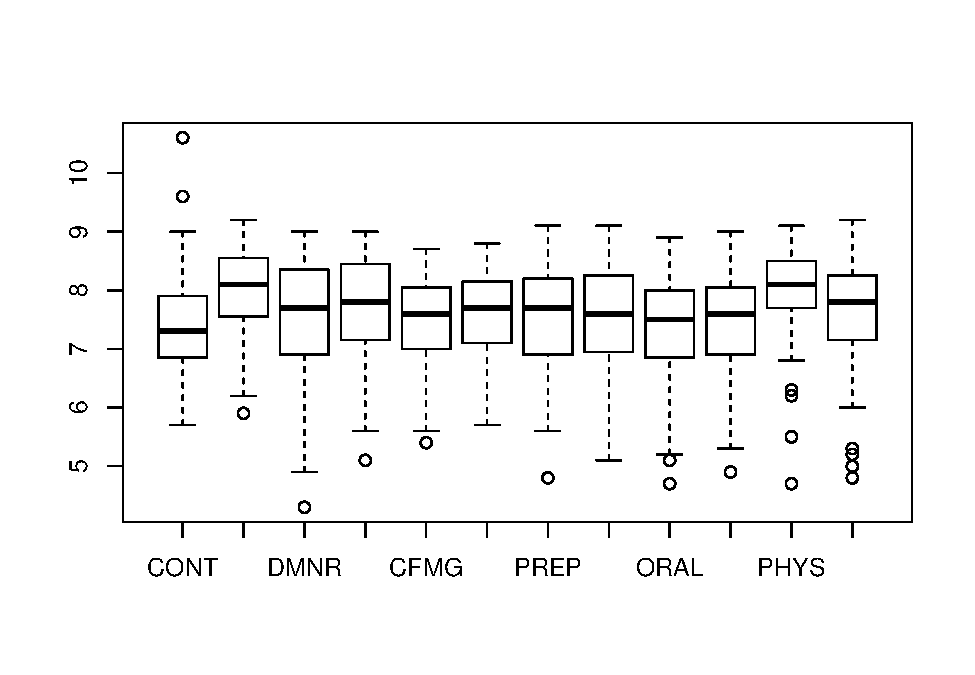
\includegraphics{Homework_Adrien_Toulouse_Paul-Antoine_Girard_files/figure-latex/boxplot-1.pdf}

We observe the presence of outliers for 10 of the 12 variables (with
larger values for CONT and with lower values for the other variables).

Let's take a closer look at these outliers.

\begin{Shaded}
\begin{Highlighting}[]
\KeywordTok{max}\NormalTok{(USJudgeRatings}\OperatorTok{$}\NormalTok{CONT)}
\end{Highlighting}
\end{Shaded}

\begin{verbatim}
## [1] 10.6
\end{verbatim}

\begin{Shaded}
\begin{Highlighting}[]
\KeywordTok{rownames}\NormalTok{(USJudgeRatings)[}\KeywordTok{which.max}\NormalTok{(USJudgeRatings}\OperatorTok{$}\NormalTok{CONT)]}
\end{Highlighting}
\end{Shaded}

\begin{verbatim}
## [1] "CALLAHAN,R.J."
\end{verbatim}

The judge with the biggest number of contacts of lawyer is judge
Callahan with a a number of 10.6 contacts.

\begin{Shaded}
\begin{Highlighting}[]
\KeywordTok{min}\NormalTok{(USJudgeRatings}\OperatorTok{$}\NormalTok{RTEN)}
\end{Highlighting}
\end{Shaded}

\begin{verbatim}
## [1] 4.8
\end{verbatim}

\begin{Shaded}
\begin{Highlighting}[]
\KeywordTok{rownames}\NormalTok{(USJudgeRatings)[}\KeywordTok{which.min}\NormalTok{(USJudgeRatings}\OperatorTok{$}\NormalTok{RTEN)]}
\end{Highlighting}
\end{Shaded}

\begin{verbatim}
## [1] "BRACKEN,J.J."
\end{verbatim}

The judge with the lowest rating for worthiness of retention is judge
Bracken with a rating of 4.8.

\begin{Shaded}
\begin{Highlighting}[]
\KeywordTok{max}\NormalTok{(USJudgeRatings}\OperatorTok{$}\NormalTok{RTEN)}
\end{Highlighting}
\end{Shaded}

\begin{verbatim}
## [1] 9.2
\end{verbatim}

\begin{Shaded}
\begin{Highlighting}[]
\KeywordTok{rownames}\NormalTok{(USJudgeRatings)[}\KeywordTok{which.max}\NormalTok{(USJudgeRatings}\OperatorTok{$}\NormalTok{RTEN)]}
\end{Highlighting}
\end{Shaded}

\begin{verbatim}
## [1] "RUBINOW,J.E."
\end{verbatim}

The judge with the highest rating for worthiness of retention is judge
Rubinow with a rating of 9.2.

We are not provided with extra information and nothing indicated that
these outliers correspond to mistakes. Thus, we will assume that they
aren't mistakes and keep them in our analysis.

The boxplots give us other relevant information on the PHYS variable.
This variable has quite a high mean compared to the others and a lower
interquartile range.

\begin{Shaded}
\begin{Highlighting}[]
\KeywordTok{library}\NormalTok{(ggplot2)}
\KeywordTok{library}\NormalTok{(dplyr)}
\end{Highlighting}
\end{Shaded}

\begin{verbatim}
## 
## Attaching package: 'dplyr'
\end{verbatim}

\begin{verbatim}
## The following object is masked from 'package:kableExtra':
## 
##     group_rows
\end{verbatim}

\begin{verbatim}
## The following objects are masked from 'package:stats':
## 
##     filter, lag
\end{verbatim}

\begin{verbatim}
## The following objects are masked from 'package:base':
## 
##     intersect, setdiff, setequal, union
\end{verbatim}

\begin{Shaded}
\begin{Highlighting}[]
\KeywordTok{library}\NormalTok{(GGally)}
\end{Highlighting}
\end{Shaded}

\begin{verbatim}
## Registered S3 method overwritten by 'GGally':
##   method from   
##   +.gg   ggplot2
\end{verbatim}

\begin{verbatim}
## 
## Attaching package: 'GGally'
\end{verbatim}

\begin{verbatim}
## The following object is masked from 'package:dplyr':
## 
##     nasa
\end{verbatim}

\begin{Shaded}
\begin{Highlighting}[]
\KeywordTok{ggpairs}\NormalTok{(USJudgeRatings)}
\end{Highlighting}
\end{Shaded}

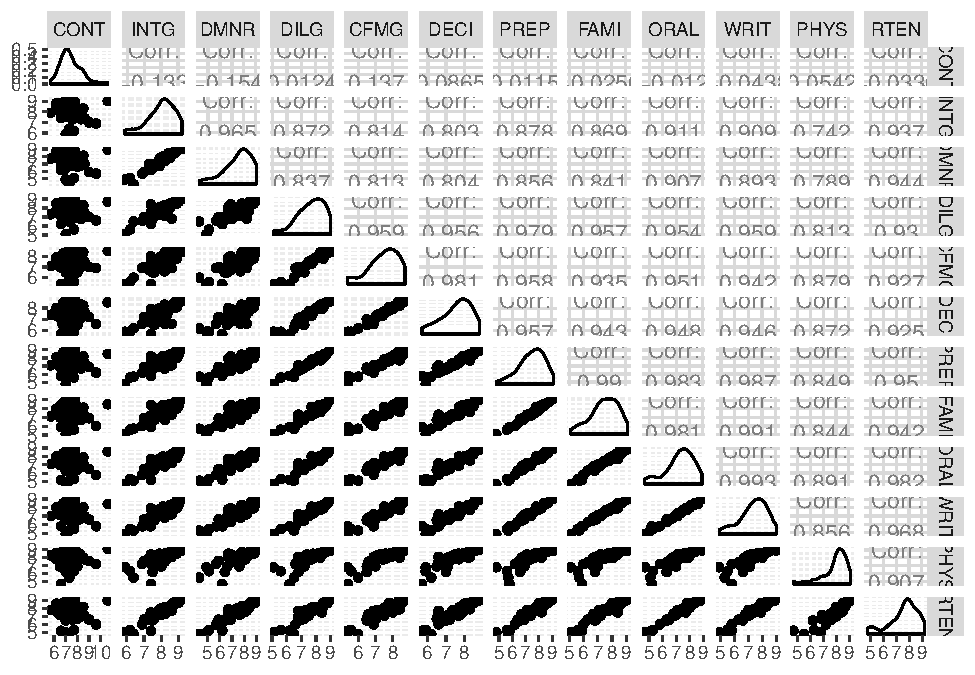
\includegraphics{Homework_Adrien_Toulouse_Paul-Antoine_Girard_files/figure-latex/unnamed-chunk-5-1.pdf}

\begin{Shaded}
\begin{Highlighting}[]
\KeywordTok{hist}\NormalTok{(USJudgeRatings}\OperatorTok{$}\NormalTok{CONT, }\DataTypeTok{main=}\StringTok{"CONT"}\NormalTok{)}
\end{Highlighting}
\end{Shaded}

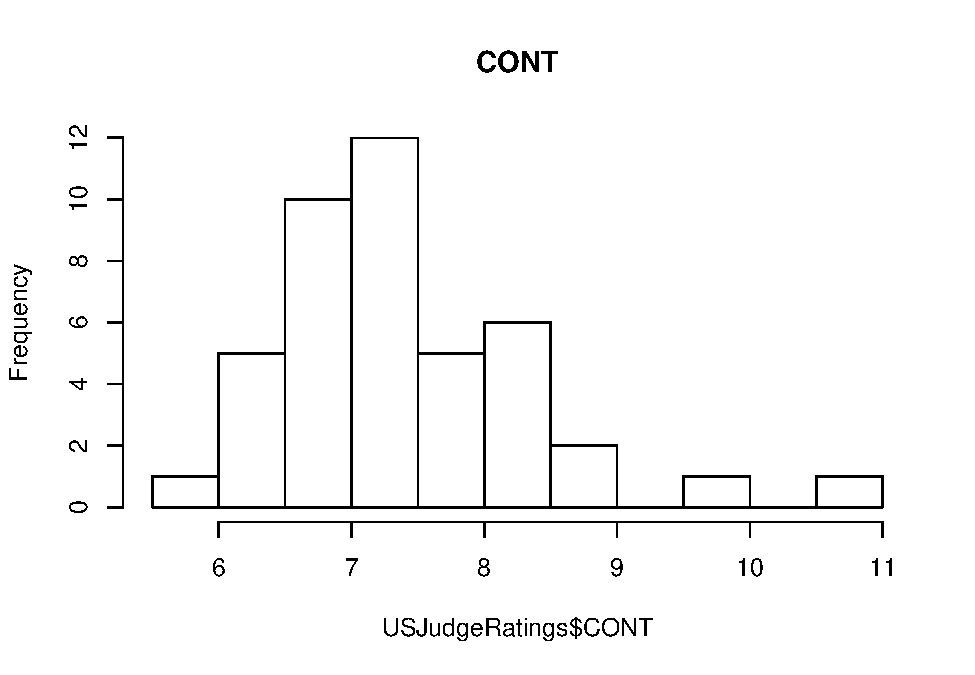
\includegraphics{Homework_Adrien_Toulouse_Paul-Antoine_Girard_files/figure-latex/histograms-1.pdf}

\begin{Shaded}
\begin{Highlighting}[]
\KeywordTok{hist}\NormalTok{(USJudgeRatings}\OperatorTok{$}\NormalTok{PREP, }\DataTypeTok{main=}\StringTok{"PREP"}\NormalTok{ )}
\end{Highlighting}
\end{Shaded}

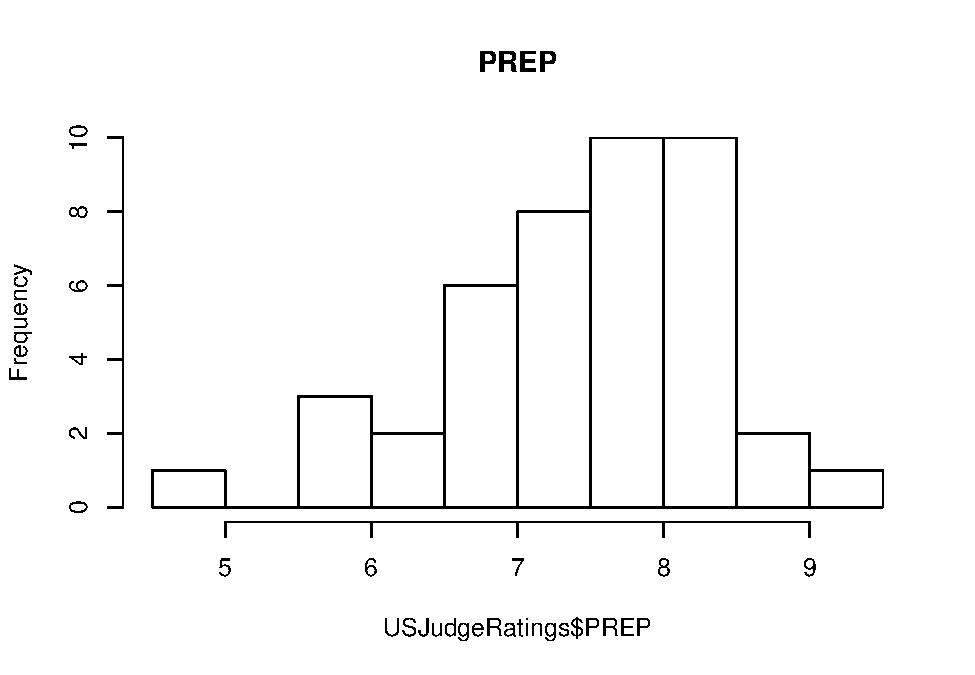
\includegraphics{Homework_Adrien_Toulouse_Paul-Antoine_Girard_files/figure-latex/unnamed-chunk-6-1.pdf}

\begin{Shaded}
\begin{Highlighting}[]
\KeywordTok{hist}\NormalTok{(USJudgeRatings}\OperatorTok{$}\NormalTok{WRIT, }\DataTypeTok{main=}\StringTok{"WRIT"}\NormalTok{)}
\end{Highlighting}
\end{Shaded}

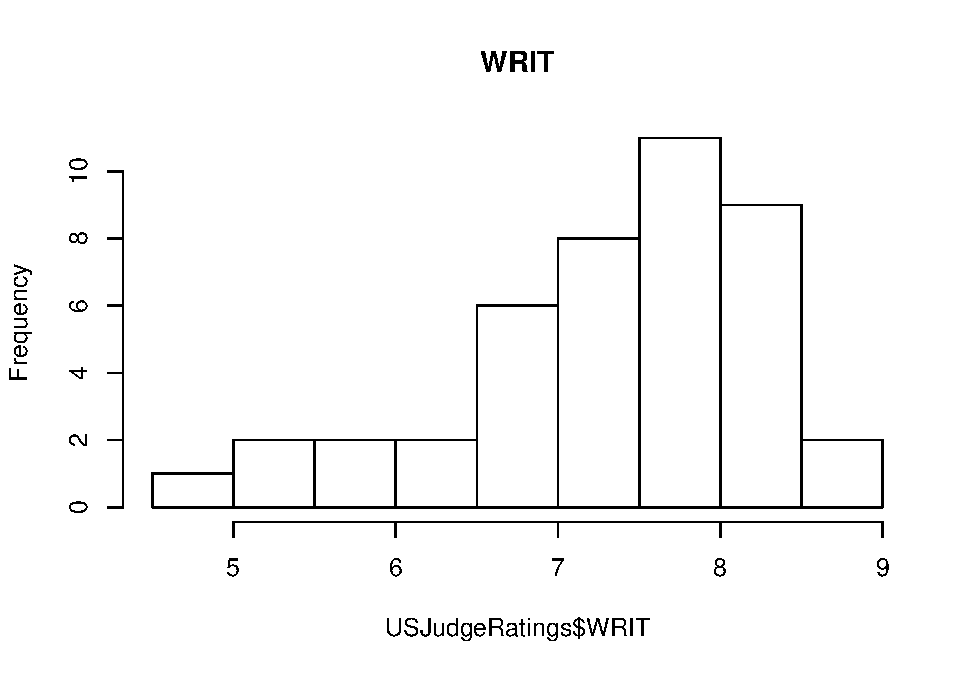
\includegraphics{Homework_Adrien_Toulouse_Paul-Antoine_Girard_files/figure-latex/unnamed-chunk-7-1.pdf}

\begin{Shaded}
\begin{Highlighting}[]
\KeywordTok{hist}\NormalTok{(USJudgeRatings}\OperatorTok{$}\NormalTok{RTEN, }\DataTypeTok{main=}\StringTok{"RTEN"}\NormalTok{)}
\end{Highlighting}
\end{Shaded}

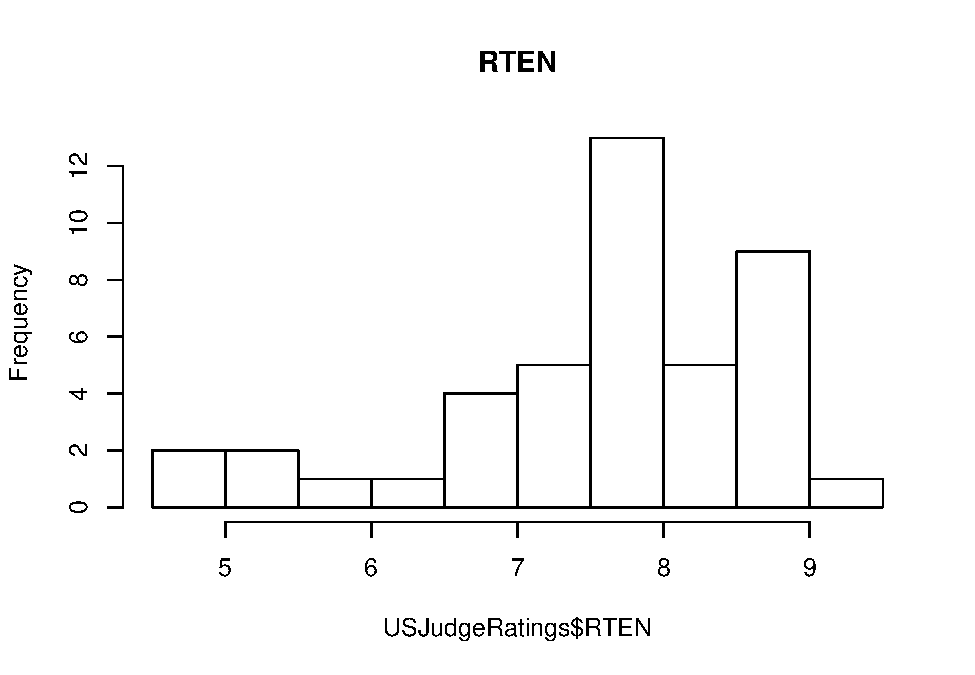
\includegraphics{Homework_Adrien_Toulouse_Paul-Antoine_Girard_files/figure-latex/unnamed-chunk-8-1.pdf}

\begin{Shaded}
\begin{Highlighting}[]
\KeywordTok{round}\NormalTok{(}\KeywordTok{var}\NormalTok{(USJudgeRatings), }\DecValTok{2}\NormalTok{)}
\end{Highlighting}
\end{Shaded}

\begin{verbatim}
##       CONT  INTG  DMNR DILG CFMG DECI PREP  FAMI  ORAL  WRIT PHYS  RTEN
## CONT  0.89 -0.10 -0.17 0.01 0.11 0.07 0.01 -0.02 -0.01 -0.04 0.05 -0.03
## INTG -0.10  0.59  0.85 0.60 0.54 0.50 0.64  0.64  0.71  0.67 0.54  0.79
## DMNR -0.17  0.85  1.31 0.86 0.80 0.74 0.93  0.91  1.05  0.98 0.85  1.19
## DILG  0.01  0.60  0.86 0.81 0.74 0.69 0.84  0.82  0.87  0.83 0.69  0.92
## CFMG  0.11  0.54  0.80 0.74 0.74 0.68 0.79  0.76  0.83  0.78 0.71  0.88
## DECI  0.07  0.50  0.74 0.69 0.68 0.64 0.73  0.72  0.77  0.73 0.66  0.82
## PREP  0.01  0.64  0.93 0.84 0.79 0.73 0.91  0.90  0.95  0.90 0.76  1.00
## FAMI -0.02  0.64  0.91 0.82 0.76 0.72 0.90  0.90  0.94  0.90 0.75  0.98
## ORAL -0.01  0.71  1.05 0.87 0.83 0.77 0.95  0.94  1.02  0.96 0.85  1.09
## WRIT -0.04  0.67  0.98 0.83 0.78 0.73 0.90  0.90  0.96  0.92 0.77  1.02
## PHYS  0.05  0.54  0.85 0.69 0.71 0.66 0.76  0.75  0.85  0.77 0.88  0.94
## RTEN -0.03  0.79  1.19 0.92 0.88 0.82 1.00  0.98  1.09  1.02 0.94  1.21
\end{verbatim}

\begin{Shaded}
\begin{Highlighting}[]
\KeywordTok{round}\NormalTok{(}\KeywordTok{sqrt}\NormalTok{(}\KeywordTok{diag}\NormalTok{(}\KeywordTok{var}\NormalTok{(USJudgeRatings))),}\DecValTok{2}\NormalTok{)}
\end{Highlighting}
\end{Shaded}

\begin{verbatim}
## CONT INTG DMNR DILG CFMG DECI PREP FAMI ORAL WRIT PHYS RTEN 
## 0.94 0.77 1.14 0.90 0.86 0.80 0.95 0.95 1.01 0.96 0.94 1.10
\end{verbatim}

\begin{Shaded}
\begin{Highlighting}[]
\KeywordTok{print}\NormalTok{(}\StringTok{'The smallest standard deviation is: '}\NormalTok{)}
\end{Highlighting}
\end{Shaded}

\begin{verbatim}
## [1] "The smallest standard deviation is: "
\end{verbatim}

\begin{Shaded}
\begin{Highlighting}[]
\KeywordTok{min}\NormalTok{(}\KeywordTok{round}\NormalTok{(}\KeywordTok{sqrt}\NormalTok{(}\KeywordTok{diag}\NormalTok{(}\KeywordTok{var}\NormalTok{(USJudgeRatings))),}\DecValTok{2}\NormalTok{))}
\end{Highlighting}
\end{Shaded}

\begin{verbatim}
## [1] 0.77
\end{verbatim}

\begin{Shaded}
\begin{Highlighting}[]
\KeywordTok{print}\NormalTok{(}\StringTok{'The largest standard deviation is: '}\NormalTok{)}
\end{Highlighting}
\end{Shaded}

\begin{verbatim}
## [1] "The largest standard deviation is: "
\end{verbatim}

\begin{Shaded}
\begin{Highlighting}[]
\KeywordTok{max}\NormalTok{(}\KeywordTok{round}\NormalTok{(}\KeywordTok{sqrt}\NormalTok{(}\KeywordTok{diag}\NormalTok{(}\KeywordTok{var}\NormalTok{(USJudgeRatings))),}\DecValTok{2}\NormalTok{))}
\end{Highlighting}
\end{Shaded}

\begin{verbatim}
## [1] 1.14
\end{verbatim}

Regarding the dispersion, we look at the interquartile range (given by
the boxplots) and the empirical standard deviation. Overall, the
dispersions are not very high (around 1). We find that the variables
DMNR and RTEN have the largest standard deviation, while the DECI
variable has the smallest.

Let's measure the correlations between the 11 first variables and the
variable RTEN. For this we use the correlations function and the pairs
function to visualize the scatter plots of the variables two by two.

\begin{Shaded}
\begin{Highlighting}[]
\KeywordTok{round}\NormalTok{(}\KeywordTok{cor}\NormalTok{(USJudgeRatings),}\DecValTok{2}\NormalTok{)}
\end{Highlighting}
\end{Shaded}

\begin{verbatim}
##       CONT  INTG  DMNR DILG CFMG DECI PREP  FAMI  ORAL  WRIT PHYS  RTEN
## CONT  1.00 -0.13 -0.15 0.01 0.14 0.09 0.01 -0.03 -0.01 -0.04 0.05 -0.03
## INTG -0.13  1.00  0.96 0.87 0.81 0.80 0.88  0.87  0.91  0.91 0.74  0.94
## DMNR -0.15  0.96  1.00 0.84 0.81 0.80 0.86  0.84  0.91  0.89 0.79  0.94
## DILG  0.01  0.87  0.84 1.00 0.96 0.96 0.98  0.96  0.95  0.96 0.81  0.93
## CFMG  0.14  0.81  0.81 0.96 1.00 0.98 0.96  0.94  0.95  0.94 0.88  0.93
## DECI  0.09  0.80  0.80 0.96 0.98 1.00 0.96  0.94  0.95  0.95 0.87  0.92
## PREP  0.01  0.88  0.86 0.98 0.96 0.96 1.00  0.99  0.98  0.99 0.85  0.95
## FAMI -0.03  0.87  0.84 0.96 0.94 0.94 0.99  1.00  0.98  0.99 0.84  0.94
## ORAL -0.01  0.91  0.91 0.95 0.95 0.95 0.98  0.98  1.00  0.99 0.89  0.98
## WRIT -0.04  0.91  0.89 0.96 0.94 0.95 0.99  0.99  0.99  1.00 0.86  0.97
## PHYS  0.05  0.74  0.79 0.81 0.88 0.87 0.85  0.84  0.89  0.86 1.00  0.91
## RTEN -0.03  0.94  0.94 0.93 0.93 0.92 0.95  0.94  0.98  0.97 0.91  1.00
\end{verbatim}

\begin{Shaded}
\begin{Highlighting}[]
\KeywordTok{library}\NormalTok{(corrplot)}
\end{Highlighting}
\end{Shaded}

\begin{verbatim}
## corrplot 0.84 loaded
\end{verbatim}

\begin{Shaded}
\begin{Highlighting}[]
\KeywordTok{corrplot}\NormalTok{(}\KeywordTok{cor}\NormalTok{(USJudgeRatings))}
\end{Highlighting}
\end{Shaded}

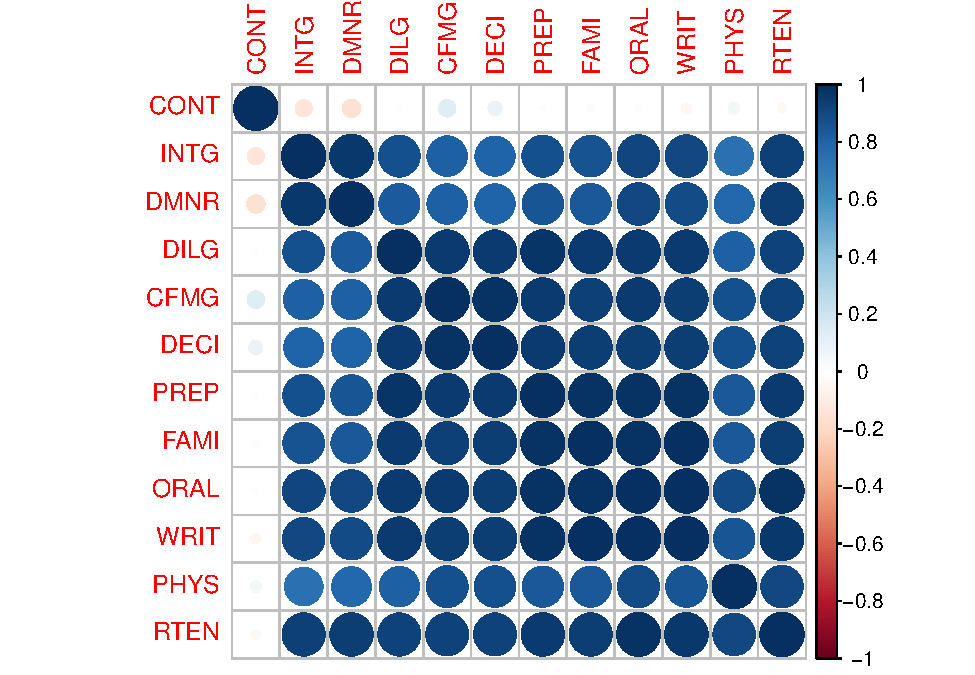
\includegraphics{Homework_Adrien_Toulouse_Paul-Antoine_Girard_files/figure-latex/linear relationships between variables 2-1.pdf}

\begin{Shaded}
\begin{Highlighting}[]
\KeywordTok{pairs}\NormalTok{(USJudgeRatings)}
\end{Highlighting}
\end{Shaded}

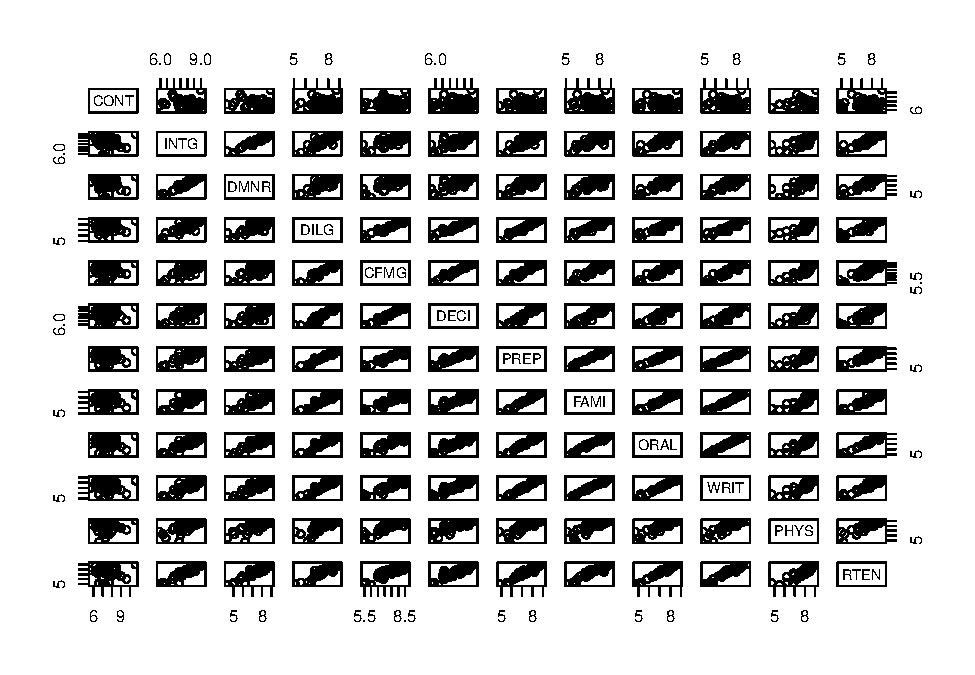
\includegraphics{Homework_Adrien_Toulouse_Paul-Antoine_Girard_files/figure-latex/pairs-1.pdf}
All the variables have a strong positive correlation two by two except
the variable CONT which is not correlated to all the other variables.
The number of contacts of a lawyer with the judge doesn't seem to
explain the ratings received by the judge.

\begin{Shaded}
\begin{Highlighting}[]
\KeywordTok{par}\NormalTok{(}\DataTypeTok{mfrow=}\KeywordTok{c}\NormalTok{(}\DecValTok{1}\NormalTok{,}\DecValTok{2}\NormalTok{))}
\KeywordTok{hist}\NormalTok{(USJudgeRatings}\OperatorTok{$}\NormalTok{CONT, }\DataTypeTok{probability=} \OtherTok{TRUE}\NormalTok{, }\DataTypeTok{main=}\StringTok{"Histogram of CONT"}\NormalTok{, }\DataTypeTok{xlab=}\StringTok{"CONT"}\NormalTok{)}
\NormalTok{d =}\StringTok{ }\KeywordTok{density}\NormalTok{(USJudgeRatings}\OperatorTok{$}\NormalTok{CONT, }\DataTypeTok{kernel =} \StringTok{'c'}\NormalTok{, }\DataTypeTok{bw =} \FloatTok{0.3}\NormalTok{)}
\KeywordTok{lines}\NormalTok{(d, }\DataTypeTok{col=}\StringTok{"red"}\NormalTok{)}

\KeywordTok{hist}\NormalTok{(USJudgeRatings}\OperatorTok{$}\NormalTok{RTEN, }\DataTypeTok{probability=} \OtherTok{TRUE}\NormalTok{, }\DataTypeTok{main=}\StringTok{"Histogram of RTEN"}\NormalTok{ , }\DataTypeTok{xlab=}\StringTok{"RTEN"}\NormalTok{)}
\NormalTok{d =}\StringTok{ }\KeywordTok{density}\NormalTok{(USJudgeRatings}\OperatorTok{$}\NormalTok{RTEN, }\DataTypeTok{kernel =} \StringTok{'o'}\NormalTok{, }\DataTypeTok{bw =} \FloatTok{0.3}\NormalTok{)}
\KeywordTok{lines}\NormalTok{(d, }\DataTypeTok{col=}\StringTok{"red"}\NormalTok{)}
\end{Highlighting}
\end{Shaded}

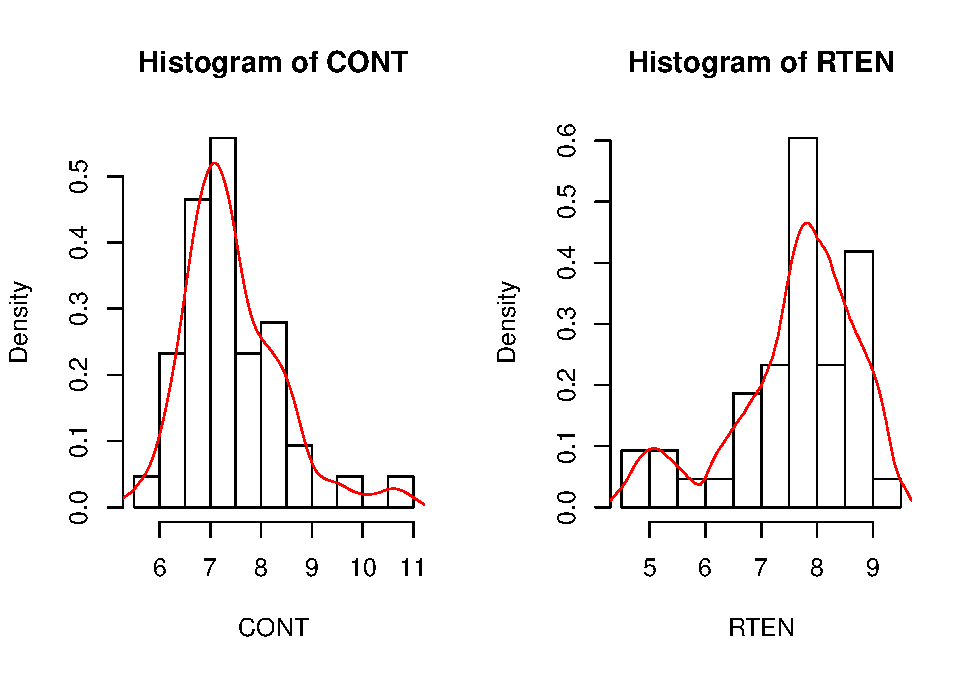
\includegraphics{Homework_Adrien_Toulouse_Paul-Antoine_Girard_files/figure-latex/density-1.pdf}

\begin{Shaded}
\begin{Highlighting}[]
\KeywordTok{par}\NormalTok{(}\DataTypeTok{mfrow=}\KeywordTok{c}\NormalTok{(}\DecValTok{1}\NormalTok{,}\DecValTok{2}\NormalTok{))}
\KeywordTok{plot}\NormalTok{(}\KeywordTok{ecdf}\NormalTok{(USJudgeRatings}\OperatorTok{$}\NormalTok{CONT), }\DataTypeTok{verticals =} \OtherTok{TRUE}\NormalTok{, }\DataTypeTok{do.points =} \OtherTok{FALSE}\NormalTok{, }\DataTypeTok{main =} \StringTok{"ECDF CONT"}\NormalTok{)}
\KeywordTok{plot}\NormalTok{(}\KeywordTok{ecdf}\NormalTok{(USJudgeRatings}\OperatorTok{$}\NormalTok{RTEN), }\DataTypeTok{verticals =} \OtherTok{TRUE}\NormalTok{, }\DataTypeTok{do.points =} \OtherTok{FALSE}\NormalTok{, }\DataTypeTok{main =} \StringTok{"ECDF RTEN"}\NormalTok{)}
\end{Highlighting}
\end{Shaded}

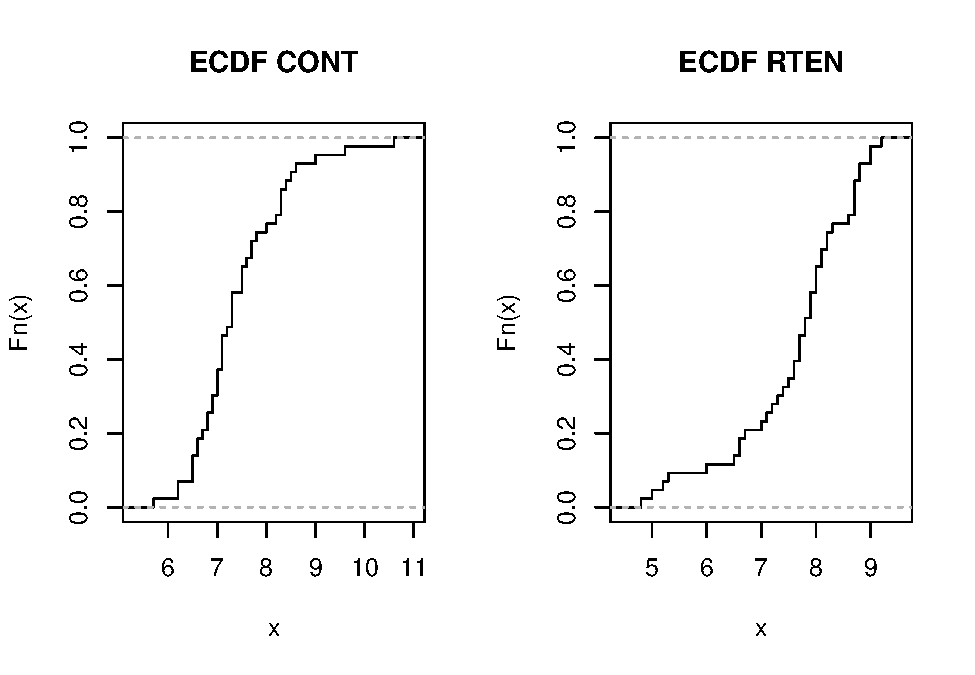
\includegraphics{Homework_Adrien_Toulouse_Paul-Antoine_Girard_files/figure-latex/ecdf-1.pdf}

\begin{Shaded}
\begin{Highlighting}[]
\KeywordTok{qqnorm}\NormalTok{(USJudgeRatings}\OperatorTok{$}\NormalTok{RTEN)}
\KeywordTok{qqline}\NormalTok{(USJudgeRatings}\OperatorTok{$}\NormalTok{RTEN)}
\end{Highlighting}
\end{Shaded}

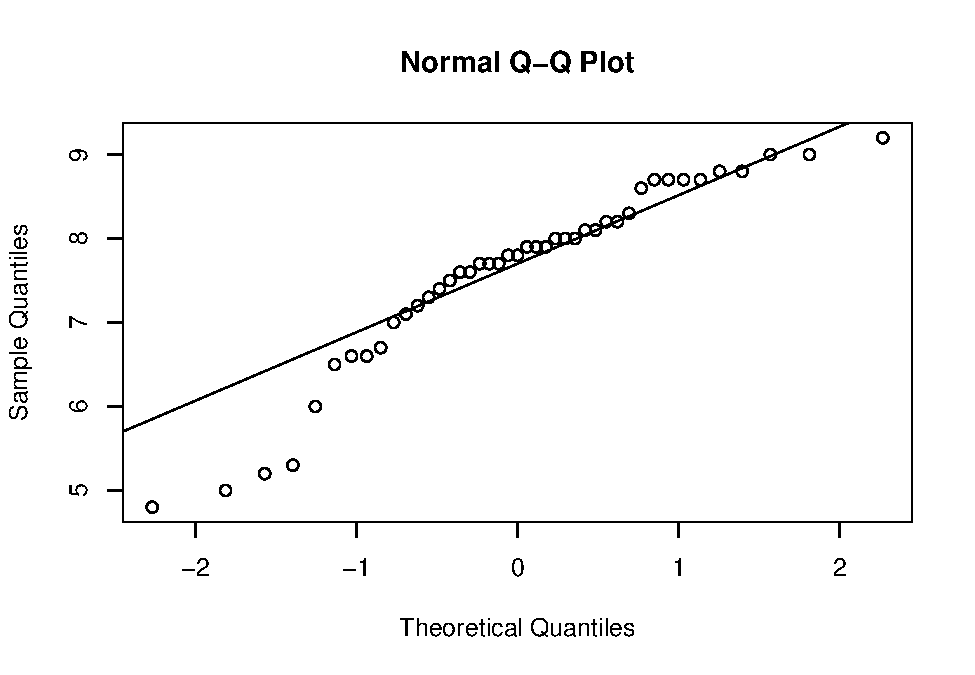
\includegraphics{Homework_Adrien_Toulouse_Paul-Antoine_Girard_files/figure-latex/QQ plot-1.pdf}
The QQ plots suggests that the RTEN variable seems to follow a Gaussian
distribution except for lower values.

\begin{Shaded}
\begin{Highlighting}[]
\KeywordTok{library}\NormalTok{(e1071)}
\KeywordTok{kurtosis}\NormalTok{(USJudgeRatings}\OperatorTok{$}\NormalTok{RTEN)}
\end{Highlighting}
\end{Shaded}

\begin{verbatim}
## [1] 0.2557421
\end{verbatim}

\begin{Shaded}
\begin{Highlighting}[]
\KeywordTok{skewness}\NormalTok{(USJudgeRatings}\OperatorTok{$}\NormalTok{RTEN)}
\end{Highlighting}
\end{Shaded}

\begin{verbatim}
## [1] -0.9373609
\end{verbatim}

Skewness and kurtosis figures for the retention variable are both
between -1 and 1 which indicates no substantial skewness or kurtosis.

\hypertarget{conclusion}{%
\subsubsection{Conclusion}\label{conclusion}}

Our analysis has


\end{document}
